\documentclass[13pt,a4paper]{extarticle}
\usepackage[utf8]{inputenc}
\usepackage[utf8]{vietnam} %Bien dich duoc tieng Viet
\usepackage{amsmath,amsfonts,amssymb} %Font toan
\usepackage{type1cm}
\usepackage{times}
\usepackage{graphicx}
\graphicspath{ {images08/} }
\usepackage{enumerate}
\usepackage{comment}
\usepackage{multicol}
\usepackage{multirow}
%\usepackage[unicode]{hyperref} %Tu dong tao bookmark
\usepackage[unicode, hidelinks=true]{hyperref}
\usepackage{indentfirst} %Thut vao dau dong o tat ca cac doan
\usepackage{listings} %Dinh dang code
\usepackage{color} %Mau sac
\usepackage[left=2.5cm,right=2.5cm,top=2.5cm,bottom=2.5cm]{geometry} %Canh lề trái - phải - trên - dưới cho tài liệu
\usepackage{longtable}
\renewcommand{\arraystretch}{1.3}

\begin{document}
\pagenumbering{gobble}
\title{\large{\textbf{BÀI CHUẨN BỊ THỰC TẬP ĐIỆN CÔNG NGHIỆP}}\\\vspace{1cm}\textbf{Bài 8}\\\vspace{.5cm}\textbf{VẬN HÀNH ĐIỀU KHIỂN HỆ THỐNG BÙ CÔNG SUẤT PHẢN KHÁNG ỨNG ĐỘNG 6 CẤP ĐIỀU KHIỂN}}
\date{Ngày 14 tháng 06 năm 2016}
%\date{\today}
\author{GVHD: Võ Minh Thiện \vspace{.6cm}\\  Nhóm SVTH: Nhóm 2 -- Tiểu nhóm 1: Thi Minh Nhựt}
\maketitle
\tableofcontents
\newpage
\pagenumbering{arabic}
\setcounter{page}{1}
\section{Máy đo điện vạn năng MFM384}
\subsection{Cài dặt đồng hồ MFM384}
\begin{list}{--}{}
\item Nhấn phím \verb|VAF| + \verb|PF| (nhấn giữ đồng thời).
\item Trang \verb|1|: Nhập password: mặc định là \verb|1000|. Di chuyển kết hợp các phím mũi tên. Nhấn phím \verb|E| để xác nhận.
\item Trang \verb|2|: Chọn số pha, ví dụ: 3 pha 4 dây. Kết hợp với các phím mũi tên. Nhấn phím \verb|E| để xác nhận.
\item Trang \verb|3|: Chọn hệ số biến dòng thứ cấp: \verb|Ct SEC|, ví dụ \verb|50/5| thì nhập là \verb|5|.
\item Trang \verb|4|: Hệ số biến dòng sơ cấp, ví dụ là \verb|50A|.
\item Trang \verb|5|: Hệ số biến áp thứ cấp, ví dụ \verb|220V|.
\item Trang \verb|6|: Hệ số biến áp sơ cấp, ví dụ \verb|3300V|.
\end{list}
\subsection{Đọc các thông số trên đồng hồ MFM384}
\begin{list}{--}{}
\item Chọn chế độ điều khiển bằng tay: nhấn phím \verb|A/M| trong 5s (đợi khi có sự thay đổi màn hình).
\item Đo điện áp: Nhấn phím \verb|V|.
\begin{list}{+}{}
\item Nhấn phím \verb|V| lần 1: hiện thị điện áp pha (dây L -- N).
\item Nhấn phím \verb|V| lần 2: hiển thị điện áp dây (dây L -- L).
\end{list}
\item Đo dòng điện: Nhấn phím \verb|I|: Dòng trong pha $A,B,C$.
\item Đo điện áp, dòng điện, hệ số công suất và tần số của từng pha.
\begin{list}{+}{}
\item Nhấn lần 1: Giá trị của pha A.
\item Nhấn lần 2: Giá trị của pha B.
\item Nhấn lần 3: Giá trị của pha C.
\item Nhấn lần 4: Giá trị trung bình của cả 3 pha.
\end{list}
\item Hệ số công suất: nhấn \verb|PF| để xem cho từng pha.
\item Xem công suất: Nhấn phím \verb|P|:
\begin{list}{+}{}
\item Nhấn lần 1: Công suất tác dụng trong từng pha.
\item Nhấn lần 2: Công suất phản kháng của từng pha.
\item Nhấn lần 3: Công suất biểu kiến của từng pha.
\item Nhấn lần 4: Xem P, Q, S của pha A.
\item Nhấn lần 5: Xem P, Q, S của pha B.
\item Nhấn lần 6: Xem P, Q, S của pha C.
\item Nhấn lần 7: Xem P, Q, S của cả 5 pha.
\end{list}
\item Xem điện năng: Nhấn phím \verb|E|.
\begin{list}{+}{}
\item Nhấn lần 1: Điện năng phản kháng $kVArh$.
\item Nhấn lần 2: Điện năng tác dụng $KWh$.
\item Nhấn lần 3: Điện năng biểu kiến $KVAh$.
\end{list}
\end{list}
\section{Bù công suất phản kháng}
\subsection{Lợi ích của bù công suất phản kháng}
\begin{list}{--}{}
\item Bù công suất phản kháng giảm tổn hao công suất.
\item Bù công suất phản kháng giảm giảm sụt áp.
\item Bù công suất phản kháng tăng khả năng mang tải của đường dây.
\item Bù công suất phản kháng tăng khả năng truyền tải của máy biến áp.
\end{list}
\subsection{Phương pháp bù công suất phản kháng}
Để nâng cao hệ số công suất cho thiết bị hoặc hệ thống, dùng:
\begin{list}{--}{}
\item Sử dụng máy bù: ưu điểm là mịn, nhưng phức tạp.
\item Sử dụng tụ bù với điều khiển ứng động: bù nhảy bậc, đơn giản sử dụng rộng rãi.
\end{list}

Bù công suất phản kháng trong mạng hạ áp:
\begin{list}{--}{}
\item Bù nền: sự dụng tụ điện với lượng bù cố định.
\item Thiết bị điều chính tụ bù: điểu chỉnh tự động hoặc liên tục khi phụ tải thay đổi.
\end{list}
\subsection{Chọn tụ bù}
Với hệ số công suất $\cos \varphi _1$ cần nâng lên hệ số công suất $\cos \varphi _2$ thì dung lượng tụ: $$ Q_{b} = P \left({\tan \varphi_1 - \tan \varphi_2}\right)$$
\subsection{Bộ điều khiển tụ bù QR -- T6}
Bộ điều khiển sẽ so sánh $\cos \varphi$ của phụ tải với ngưỡng đóng cắt (đã lập trình) để tiến hành đóng cắt tụ bù. Mặc định ở chế độ đóng cắt tự động.
\subsection{Cài đặt thông số bù cho bộ điều khiển QR -- T6}
Nhấn nút \verb|Mode/Prog| khoảng 2s: chọn các thông số $A,b,C,d$ và các giá trị $1,2,3,4$:
\begin{list}{--}{}
\item Ngưỡng đóng $A$: $A-1:\cos \varphi  = 0.85$ (tính cảm); $A-2:\cos \varphi  = 0.90$ (tính cảm); $A-3:\cos \varphi  = 0.95$ (tính cảm).
\item Ngưỡng cắt $b$: $b-1:\cos \varphi  = 0.95$ (tính cảm); $b-2:\cos \varphi  = 1.0$; $b-3:\cos \varphi  = 0.95$ (tính dung).
\item Thời gian đóng $C$: $C-1:5s$; $C-2:10s$; $C-3:20$; $C-4:40$.
\item Thời gian cắt $d$: $d-1:30s$; $d-2:60s$; $d-3:90s$; $d-4:120s$.
\item[$\ast$] Sau khoảng thời gian cài đặt, bộ điều khiển sẽ tác động đóng hoặc cắt.
\item Nhấn nút \verb|Mode/Prog| để lưu lại cài đặt.
\end{list}
\section{Nội dung thực hành}
\subsection{Sơ đồ mạch}
\begin{figure}[!h]
\begin{center}
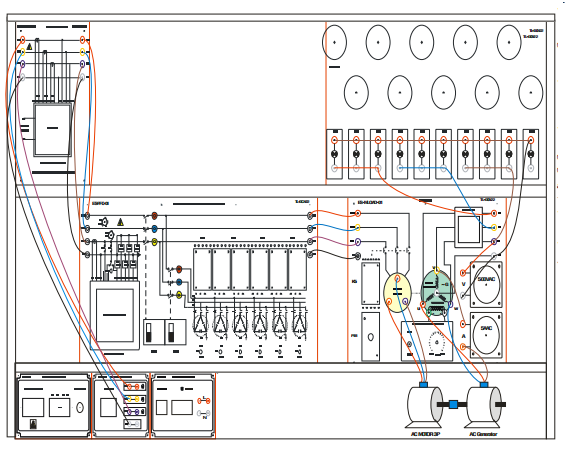
\includegraphics[scale=.8]{1}
\end{center}
\caption{Sơ đồ điều khiển tụ bù với bộ QR -- T6}
\end{figure}
\subsection{Khởi động hệ thống và đo thông số điện}\label{Sub:khoi-dong}
\begin{list}{--}{}
\item Chuyển sang chế độ \verb|Man| (gạt công tắc \verb|Auto/Man|).
\item Cấp nguồn cho hệ thống: nhấn nút \verb|Start| kiểm tra hoạt động của động cơ.
\item Xác định các thông số điện áp pha, điện áp dây, dòng điện pha, tần số, công suất phản kháng, công suất tác dụng, công suất biểu kiến, điện năng tác dụng, điện năng phản kháng đọc giá trị trên đồng hồ $MFM384$.
\end{list}
\subsection{Thực hành vận hành tụ bù bằng tay với tải cố định}
\begin{list}{--}{}
\item Thực hiện tiếp theo các bước ở mục \ref{Sub:khoi-dong}.
\item Khi động cơ đã chạy ổn định, đóng CB nối tải (các bóng đèn) nối với máy phát AC.
\item Kích từ cho máy phát: vận biến trỏ $DC1$ để $I = 2A$.
\item[$\ast$] Ở bước này nên điều chỉnh biến trở $DC1$ để dòng $I=1A,3A,4A$ phục vụ cho thí nghiệm bù tự động khi tải thay đổi, ghi nhận giá trị khi chưa bù rồi điều chỉnh $I=2A$ để thực hiện tiếp thí nghiệm điều chỉnh khi tải cố định.
\item Ghi kết quả đo được của các thông số lúc chưa bù.
\item Mắc 6 công tắc $K1\div K6$ song song với tiếp điểm khởi động từ (bù song song $C = C_1 + C_2 + \cdots$), lần lượt đóng các tụ và ghi lại các thông số:
\begin{list}{+}{}
\item Đóng $K1$.
\item Đóng $K1+K2$.
\item Đóng $K1+K2+K3$.
\item Đóng $K1+K2+K3+K4$.
\item Đóng $K1+K2+K3+K4+K5$.
\item Đóng $K1+K2+K3+K4+K5+K6$.
\end{list}
\end{list}
\subsection{Thực hành thay đổi tụ bù với tải thay đổi}
\begin{list}{--}{}
\item Đặt công tắc $K1-K4$: $OFF$.
\item Chuyển về chế độ $Auto$.
\item Cấp nguồn, khởi động động cơ chạy ổn đinh.
\item Bật CB nối tải với máy phát.
\item Kích từ cho máy phát: vận biến trở $DC1$ lần lượt $I=1A,2A,3A,4A$.
\item Ghi nhận các thông số chưa bù và lúc đã bù (ở mỗi giá trị dòng điện tương ứng).
\end{list}
\end{document}